\section*{Appendix}
\subsection*{Strict Semantics}
\begin{frame}<10>[t]
\subsectionpage\vskip 9pt
\ref{def:ss}\hspace{14.5mm}{\color{seeblau100}Sobel Sequence schematic}~~~~~~~~~~~~~~~~/~~~{\color{seeblau100}Reverse Sobel Sequence schematic}\\
\phantom{\ref*{def:ss}}\hspace{14.5mm}If $\color{red}\phi$ then $\color{OliveGreen}\chi$, but if $({\color{red}\phi}\land{\color{Orange}\psi})$ then not $\color{OliveGreen}\chi$~~~/~~~If $({\color{red}\phi}\land{\color{Orange}\psi})$ then not $\color{OliveGreen}\chi$, but if $\color{red}\phi$ then $\color{OliveGreen}\chi$\vskip 9.25pt\vskip 18pt

        \begin{itemize}
            \item<3-> Strict Analyses \citep{Peirce1896,Lewis1912,Lewis1914,Lewis1918}
        \end{itemize}
\vskip 9pt
\visible<5->{\begin{myframe}[top=5pt,bottom=5pt,left=5pt,right=5pt,arc=5pt,auto outer arc]
{\begin{minipage}[h]{\textwidth}
\ex.	For all contexts $c$, `If $\color{red}\phi$, then $\color{OliveGreen}\chi$' is true at $w$ in $c$ iff \textbf{all $\color{red}\phi$-worlds in a domain D}\linebreak\phantom{For all contexts $c$,} are $\color{OliveGreen}\chi$-worlds, where D is the set of all possible worlds.\label{def:strict}

\end{minipage}}
\end{myframe}}
\end{frame}

\begin{frame}<10>[t]
\subsectionpage\vskip 9pt
\begin{itemize}
    \item `All ${\color{red}\phi}\land{\color{Orange}\psi}$-worlds' is a subset of `all $\color{red}\phi$-worlds'
\end{itemize}\vskip 9pt
\begin{figure}[ht!]
\centering
\begin{tikzpicture}
    \coordinate (center) at (0,0);
    \fill[seeblau100] (center) + (0, 2) arc (90:360:2);
    \fill[seeblau100] (center) + (0, -2) arc (270:450:2);
    \draw circle (2);
    \draw[color=white,fill=white] circle (0.4);
    \node {w$_0$};
	\node at (-0.85,0) {w$_1$};
	\node at (-1.25,0.75) {w$_2$};
	\node at (-1.25,-0.75) {w$_3$};
	\node at (0.85,0) {w$_4$};
	\node at (1.25,0.75) {w$_5$};
	\node at (1.25,-0.75) {w$_6$};
    \node at (0,-2.5) {If $\color{red}\phi$, then $\color{OliveGreen}\chi$};
    \draw[color=seeblau100,line width=2mm,>={Triangle[length=4mm,width=4mm]},->] (2.5,0) -- (3.5,0);
    \begin{scope}[xshift=6cm]
    \coordinate (center) at (0,0);
    \fill[seeblau100] (center) + (0, -2) arc (270:450:2);
    \draw circle (2);
    \draw[color=white,fill=white] circle (0.4);
    \node {w$_0$};
	\node at (-0.85,0) {w$_1$};
	\node at (-1.25,0.75) {w$_2$};
	\node at (-1.25,-0.75) {w$_3$};
	\node at (0.85,0) {w$_4$};
	\node at (1.25,0.75) {w$_5$};
	\node at (1.25,-0.75) {w$_6$};
    \node at (0,-2.5) {If ${\color{red}\phi}\land{\color{Orange}\psi}$, then not $\color{OliveGreen}\chi$};
	\node at (3,0) {\textbf{VS}};

	\begin{scope}[xshift=6cm]
	\coordinate (center) at (0,0);
    \fill[seeblau100] (center) + (0, -2) arc (270:450:2);
    \draw circle (2);
    \draw[color=white,fill=white] circle (0.4);
    \node {w$_0$};
	\node at (-0.85,0) {w$_1$};
	\node at (-1.25,0.75) {w$_2$};
	\node at (-1.25,-0.75) {w$_3$};
	\node at (0.85,0) {w$_4$};
	\node at (1.25,0.75) {w$_5$};
	\node at (1.25,-0.75) {w$_6$};
    \node at (0,-2.5) {If ${\color{red}\phi}\land{\color{Orange}\psi}$, then not $\color{OliveGreen}\chi$};

    \draw[color=seeblau100,line width=2mm,>={Triangle[length=4mm,width=4mm]},->] (2.5,0) -- (3.5,0);
 
	\begin{scope}[xshift=6cm]
	\coordinate (center) at (0,0);
    \fill[seeblau100] (center) + (0, 2) arc (90:360:2);
    \fill[seeblau100] (center) + (0, -2) arc (270:450:2);
    \draw circle (2);
    \draw[color=white,fill=white] circle (0.4);
    \node {w$_0$};
	\node at (-0.85,0) {w$_1$};
	\node at (-1.25,0.75) {w$_2$};
	\node at (-1.25,-0.75) {w$_3$};
	\node at (0.85,0) {w$_4$};
	\node at (1.25,0.75) {w$_5$};
	\node at (1.25,-0.75) {w$_6$};
    \node at (0,-2.5) {If $\color{red}\phi$, then $\color{OliveGreen}\chi$};
	\end{scope}
	\end{scope}
	\end{scope}
\end{tikzpicture}
\end{figure}
\begin{itemize}
    \item Either sequence type would be contradictory
\end{itemize}
\end{frame}

\subsection*{Karen Lewis (2018)}
\begin{frame}<10->[t]
	\subsectionpage	\vskip 9pt
	\begin{itemize}
		\item<1->	\citepos{Lewis2017} missing factor: varying degrees of inter-antecedental similarity\vskip 18pt
		    \begin{itemize}
		        %
		        \item<3-> World closeness orderings are dynamic \citep{Lewis2016}\vskip 9pt
		        \item<4-> World closeness = Similarity $\times$ Relevance \citep{Lewis2016}\vskip 9pt
		        \item<5-> Antecedent worlds relevance is increased post-utterance \citep{Lewis2017}
		    \end{itemize}\vskip 18pt
	\end{itemize}
\end{frame}

\begin{frame}<10>[t]
\subsectionpage\vskip 9pt
\begin{itemize}
    \item If ${\color{red}\phi}\land{\color{Orange}\psi}$-worlds and $\color{red}\phi$-worlds are dissimilar to one another
\end{itemize}\vskip 9pt
\begin{figure}[ht!]
\centering
\resizebox{!}{175pt}{\begin{tikzpicture}
		\coordinate (O) at (0,0);

	\draw[fill=seeblau100] (O) circle (2.8);
	\draw[fill=white] (O) circle (2);
	\draw[fill=white] (O) circle (1.2);
	\draw[fill=white] (O) circle (0.4)node {w$_0$};

	\node at (0,0.7) {w$_1$};
	\node at (0.6,-0.5) {w$_2$};
	\node at (-0.6,-0.5) {w$_3$};
	
	\node at (0,-2.4) {w$_6$};
	\node at (-1.3,2) {w$_4$};
	\node at (1.3,2) {w$_5$};
	
	\node at (0,-3.5) {If ${\color{red}\phi}\land{\color{Orange}\psi}$, then not $\color{OliveGreen}\chi$};
	\draw[color=seeblau100,line width=2mm,>={Triangle[length=4mm,width=4mm]},->] (3,0) -- (5,0);
	
	\begin{scope}[xshift=8cm]
		\coordinate (O) at (0,0);

    \draw[fill=white] (O) circle (2.8);
	\draw[fill=white] (O) circle (2);
	\draw[fill=white] (O) circle (1.2);
	\draw[fill=white] (O) circle (0.4)node {w$_0$};

	\node at (0,0.7) {{w$_1$}};
	\node at (0.6,-0.5) {{w$_2$}};
	\node at (-0.6,-0.5) {{w$_3$}};
	
	\node at (0,-2.4) {w$_6$};
	\node at (-1.3,2) {w$_4$};
	\node at (1.3,2) {w$_5$};
	
	\draw[color=seeblau100,line width=1mm,>={Triangle[length=4mm,width=3mm]},->] (0,-2.1) -- (0,-1);
	\draw[color=seeblau100,line width=1mm,>={Triangle[length=4mm,width=3mm]},->] (-1.5,1.7) -- (-0.7,0.5);
	\draw[color=seeblau100,line width=1mm,>={Triangle[length=4mm,width=3mm]},->] (1.5,1.7) -- (0.7,0.5);
	
	\node at (0,-3.5) {Salience of ${\color{red}\phi}\land{\color{Orange}\psi}$};
	\draw[color=seeblau100,line width=2mm,>={Triangle[length=4mm,width=4mm]},->] (3,0) -- (5,0);
	
	\begin{scope}[xshift=8cm]
		\coordinate (O) at (0,0);

    \draw[fill=white] (O) circle (2.8);
	\draw[fill=white] (O) circle (2);
	\draw[fill=seeblau100] (O) circle (1.2);
	\draw[fill=white] (O) circle (0.4)node {w$_0$};

	\node at (0,0.7) {{w$_1$}};
	\node at (0.6,-0.5) {{w$_2$}};
	\node at (-0.6,-0.5) {{w$_3$}};
	
	\node at (0,-1.6) {w$_6$};
	\node at (-1,1.2) {w$_4$};
	\node at (1,1.2) {w$_5$};
	
	\node at (0,-3.5) {If $\color{red}\phi$, then $\color{OliveGreen}\chi$};
	\end{scope}
	\end{scope}
\end{tikzpicture}}
\end{figure}
\begin{itemize}
    \item No contradiction
\end{itemize}
\end{frame}

\begin{frame}<10>[t]
\subsectionpage\vskip 9pt
\begin{itemize}
    \item If ${\color{red}\phi}\land{\color{Orange}\psi}$-worlds and $\color{red}\phi$-worlds are similar to one another
\end{itemize}\vskip 9pt
\begin{figure}[ht!]
\centering
\resizebox{!}{175pt}{\begin{tikzpicture}
		\coordinate (O) at (0,0);

	\draw[fill=white] (O) circle (2.8);
	\draw[fill=seeblau100] (O) circle (2);
	\draw[fill=white] (O) circle (1.2);
	\draw[fill=white] (O) circle (0.4)node {w$_0$};

	\node at (0,0.7) {w$_1$};
	\node at (0.6,-0.5) {w$_2$};
	\node at (-0.6,-0.5) {w$_3$};
	
	\node at (0,-1.6) {w$_6$};
	\node at (-1,1.2) {w$_4$};
	\node at (1,1.2) {w$_5$};
	
	\node at (0,-3.5) {If ${\color{red}\phi}\land{\color{Orange}\psi}$, then not $\color{OliveGreen}\chi$};
	\draw[color=seeblau100,line width=2mm,>={Triangle[length=4mm,width=4mm]},->] (3,0) -- (5,0);
	
	\begin{scope}[xshift=8cm]
		\coordinate (O) at (0,0);

    \draw[fill=white] (O) circle (2.8);
	\draw[fill=white] (O) circle (2);
	\draw[fill=white] (O) circle (1.2);
	\draw[fill=white] (O) circle (0.4)node {w$_0$};

	\node at (0,0.7) {{w$_1$}};
	\node at (0.6,-0.5) {{w$_2$}};
	\node at (-0.6,-0.5) {{w$_3$}};
	
	\node at (0,-1.6) {w$_6$};
	\node at (-1,1.2) {w$_4$};
	\node at (1,1.2) {w$_5$};
	
	\draw[color=seeblau100,line width=1mm,>={Triangle[length=4mm,width=3mm]},->] (0,-2.1) -- (0,-1);
	\draw[color=seeblau100,line width=1mm,>={Triangle[length=4mm,width=3mm]},->] (-1.5,1.7) -- (-0.7,0.5);
	\draw[color=seeblau100,line width=1mm,>={Triangle[length=4mm,width=3mm]},->] (1.5,1.7) -- (0.7,0.5);
	
	\node at (0,-3.5) {Salience of ${\color{red}\phi}\land{\color{Orange}\psi}$};
	\draw[color=seeblau100,line width=2mm,>={Triangle[length=4mm,width=4mm]},->] (3,0) -- (5,0);
	
	\begin{scope}[xshift=8cm]
		\coordinate (O) at (0,0);

    \draw[fill=white] (O) circle (2.8);
	\draw[fill=white] (O) circle (2);
	\draw[fill=seeblau100] (O) circle (1.2);
	\draw[fill=white] (O) circle (0.4)node {w$_0$};

	\node at (0,0.7) {{w$_1$}};
	\node at (0.6,-0.5) {{w$_2$}};
	\node at (-0.6,-0.5) {{w$_3$}};
	
	\node at (0.1,-0.8) {w$_6$};
	\node at (-0.7,0.3) {w$_4$};
	\node at (0.7,0.3) {w$_5$};
	
	\node at (0,-3.5) {\#If $\color{red}\phi$, then $\color{OliveGreen}\chi$};
	\end{scope}
	\end{scope}
\end{tikzpicture}}
\end{figure}
\begin{itemize}
    \item Contradiction
\end{itemize}
\end{frame}

\subsection*{Ippolito (2020)}
\begin{frame}[t]
\subsectionpage\vskip 9pt\vfill
\begin{figure}
    \centering
    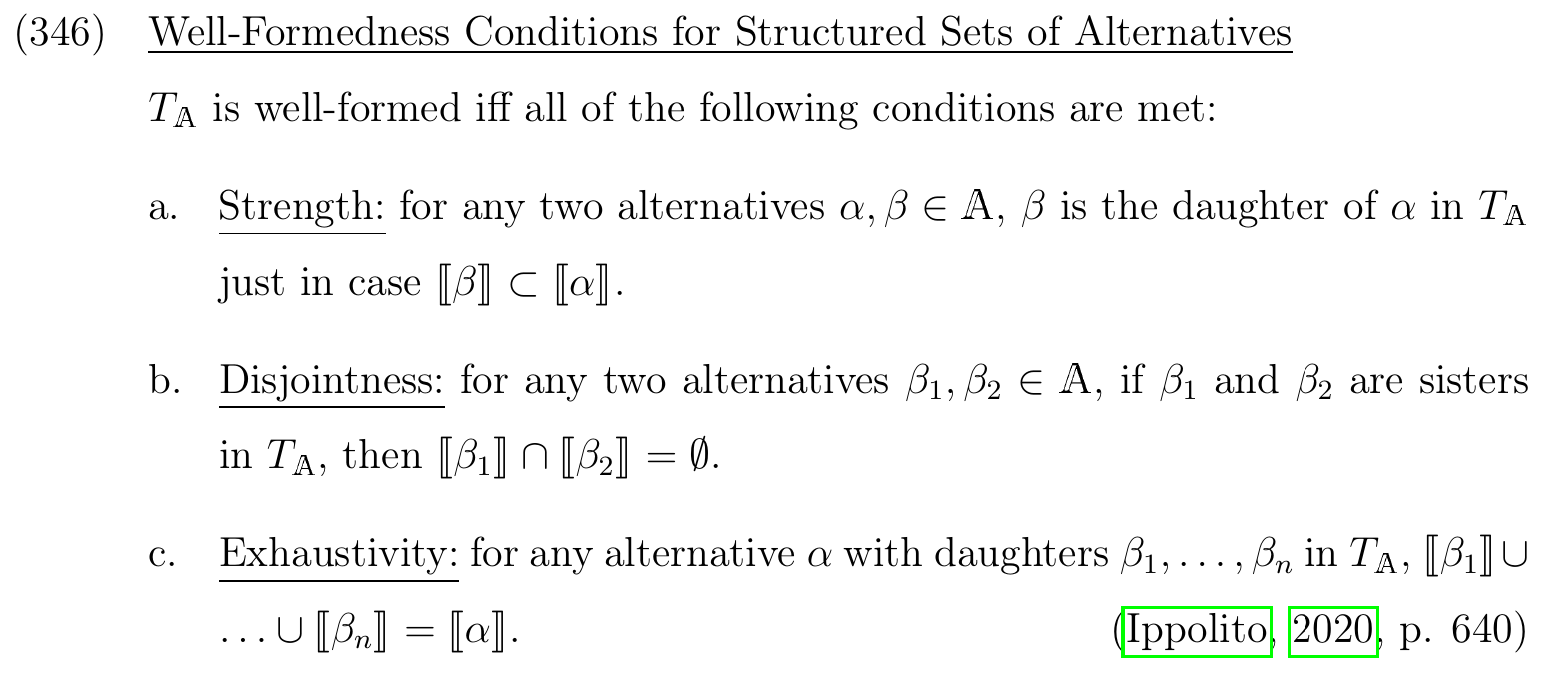
\includegraphics[width=0.8\textwidth]{graphics/ippolito-conditions.png}
\end{figure}\vfill
\end{frame}

\begin{frame}[t]
\subsectionpage\vskip 9pt\vfill
\begin{figure}
    \centering
    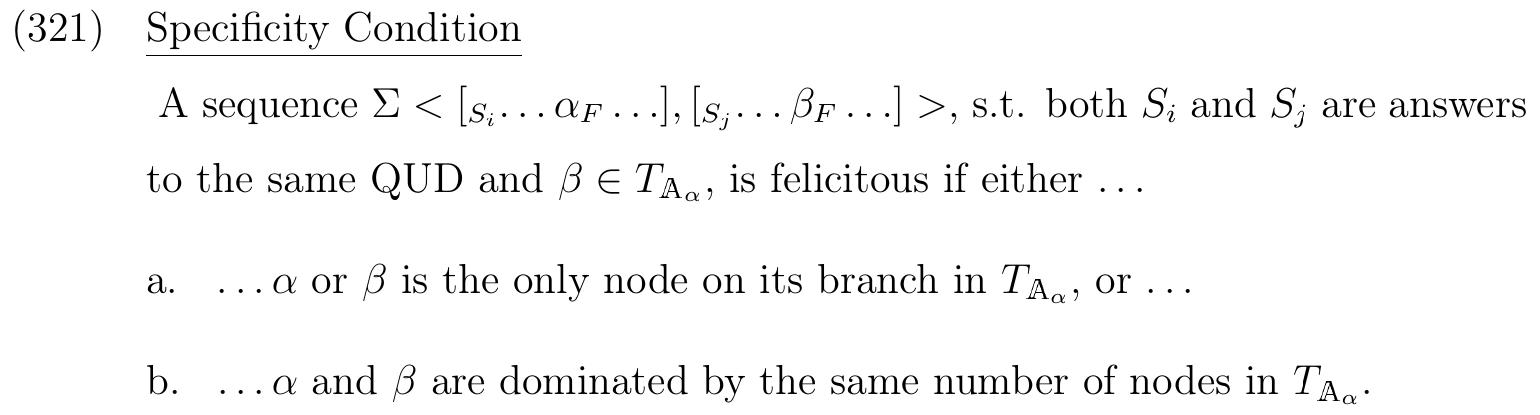
\includegraphics[width=0.8\textwidth]{graphics/ippolito-specificity.png}
\end{figure}\vfill
\end{frame}

\begin{frame}[t]
\subsectionpage\vskip 9pt\vfill
\begin{figure}
    \centering
    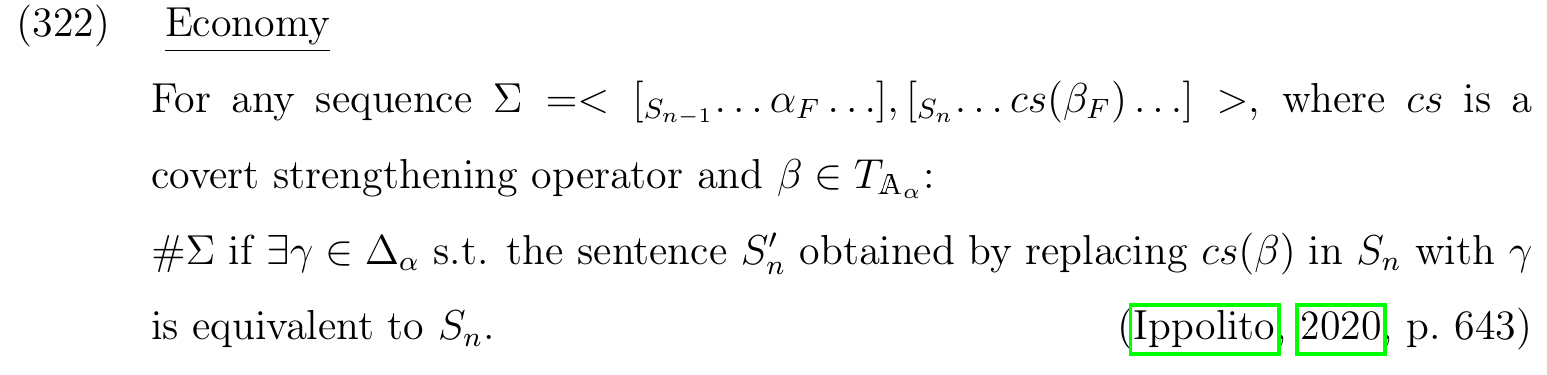
\includegraphics[width=0.8\textwidth]{graphics/ippolito-economy.png}
\end{figure}\vfill
\end{frame}

\begin{frame}[t]
\subsectionpage\vskip 9pt\vfill
\ex. John ate some or all of the cookies.

\ex. \#John ate all or some of the cookies.

\vfill
\begin{figure}
    \centering
    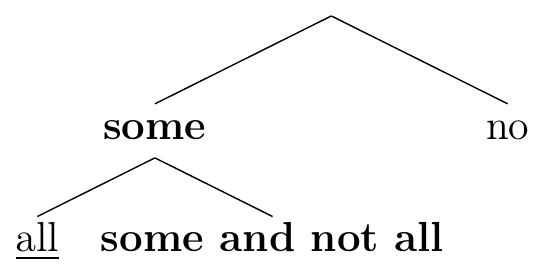
\includegraphics[width=0.3333\textwidth]{graphics/ippolito-someall-tree.png}
    \caption{Structured set of alternatives for some-but-not-all strenghtening.}
\end{figure}\vfill
\end{frame}

\begin{frame}[t]
\subsectionpage\vskip 9pt
\begin{itemize}
    \item World similarity relativised to focus value of conditional's antecedent
\end{itemize}\vfill
\begin{figure}
    \centering
    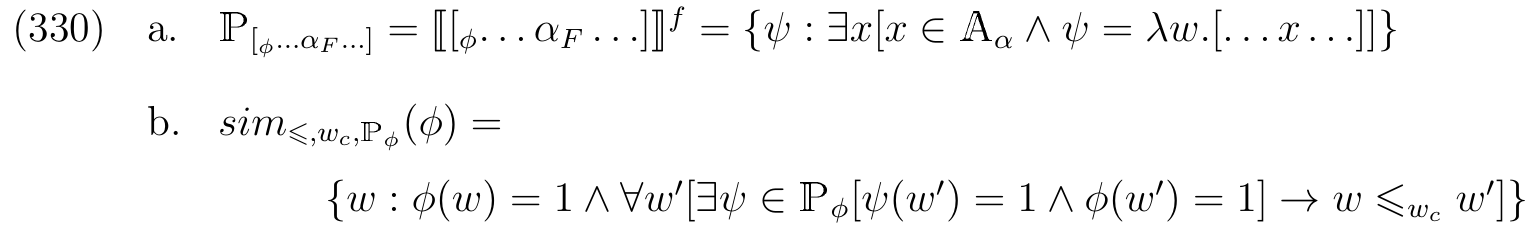
\includegraphics[width=0.8\textwidth]{graphics/ippolito-conditional-semantics.png}
\end{figure}\vfill
\end{frame}

\begin{frame}[t]
\subsectionpage\vskip 9pt\vfill
\begin{figure}
    \centering
    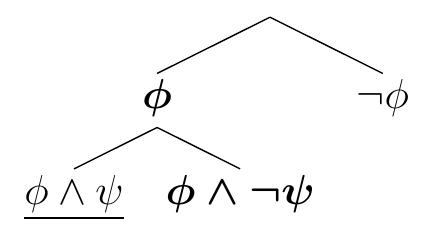
\includegraphics[width=0.3333\textwidth]{graphics/ippolito-general-rss-tree.png}
    \caption{Generalised structured set of alternatives for reverse Sobel sequences}
\end{figure}\vfill
\end{frame}

\begin{frame}[t]
\subsectionpage\vskip 9pt\vfill
\begin{figure}
    \centering
    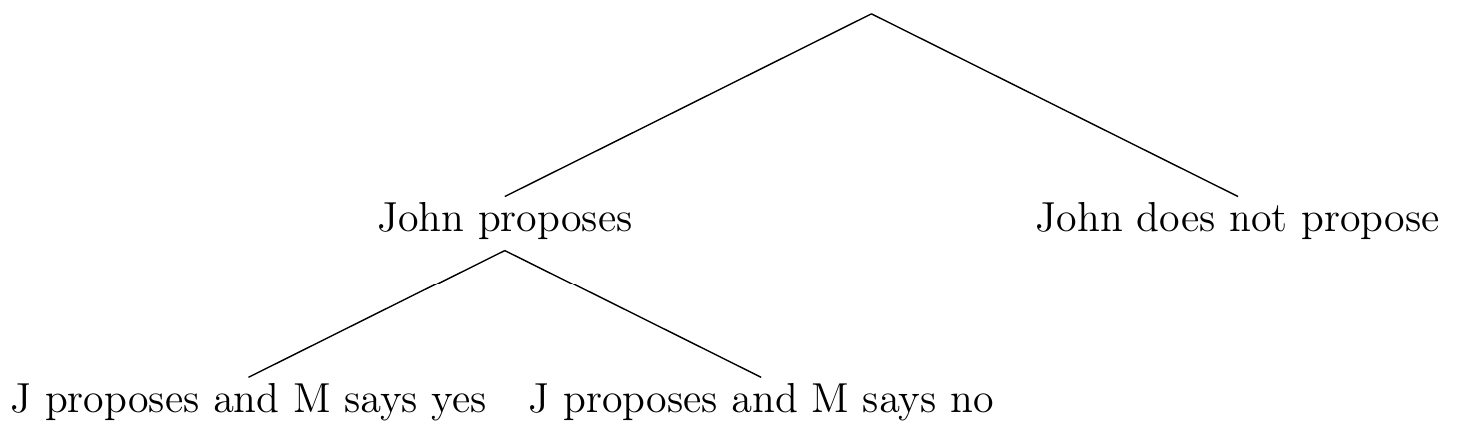
\includegraphics[width=0.9\textwidth]{graphics/ippolito-rss-prerestructure.png}
    \caption{Structured set of alternatives for $\phi\land\psi$-conditional}
\end{figure}\vfill
\end{frame}

\begin{frame}[t]
\subsectionpage\vskip 9pt\vfill
\begin{figure}
    \centering
    
\includegraphics[width=0.6666\textwidth]{graphics/ippolito-rss-postrestructure.png}
    \caption{Restructured set of alternatives for $\phi$-conditional (epistemic exclusion)}
\end{figure}\vfill
\end{frame}

\begin{frame}[t]
\subsectionpage\vskip 9pt\vfill
\begin{figure}
    \centering
    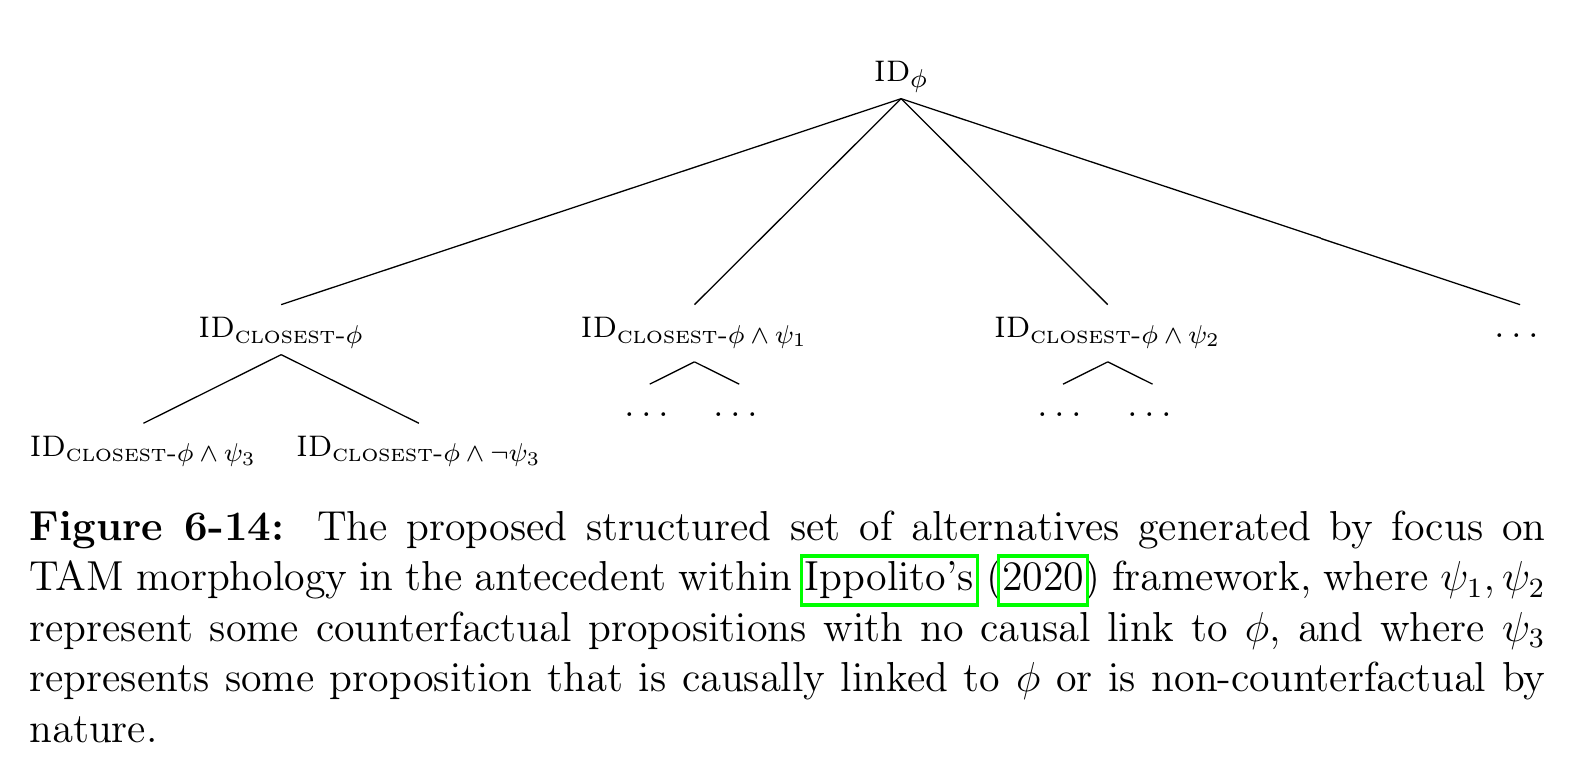
\includegraphics[trim=0 260 0 0,clip,width=0.9\textwidth]{graphics/ippolito-hybridtree.png}
    \caption{Structured set of alternatives for TAM-contrastive stress}
\end{figure}\vfill
\end{frame}

\subsection{\textit{Even}-Based NPIs}
\begin{frame}[t]
    \subsectionpage\vskip 9pt\vfill
\begin{figure}
    \centering
    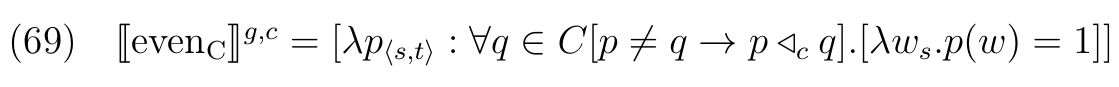
\includegraphics[width=0.7\textwidth]{graphics/crnic-even.png}
\end{figure}\vfill
\end{frame}

\begin{frame}[t]
    \subsectionpage\vskip 9pt\vfill
\begin{figure}
    \centering
    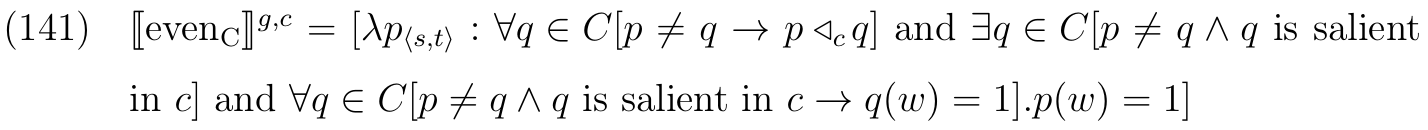
\includegraphics[width=0.8\textwidth]{graphics/crnic-even-extended.png}
\end{figure}\vfill
\end{frame}

\subsection{Crnic's SDM Context-Sensitivity}
\begin{frame}[t]
    \subsectionpage\vskip 9pt\vfill
\begin{figure}
    \centering
    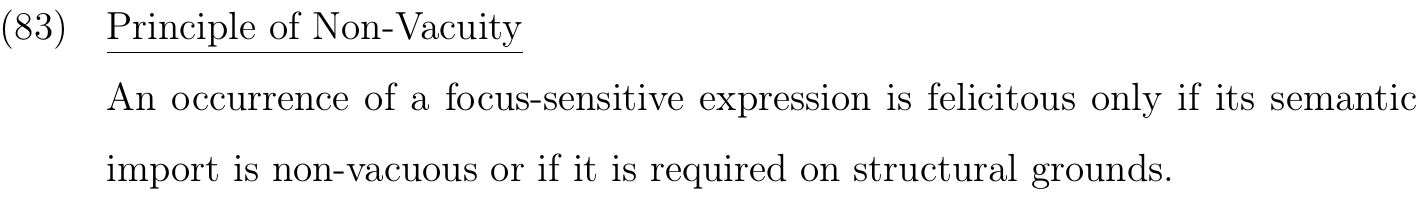
\includegraphics[width=0.8\textwidth]{graphics/crnic-nonvacuity.png}
\end{figure}\vfill
\end{frame}

\begin{frame}[t]
    \subsectionpage\vskip 9pt\vfill
\begin{figure}
    \centering
    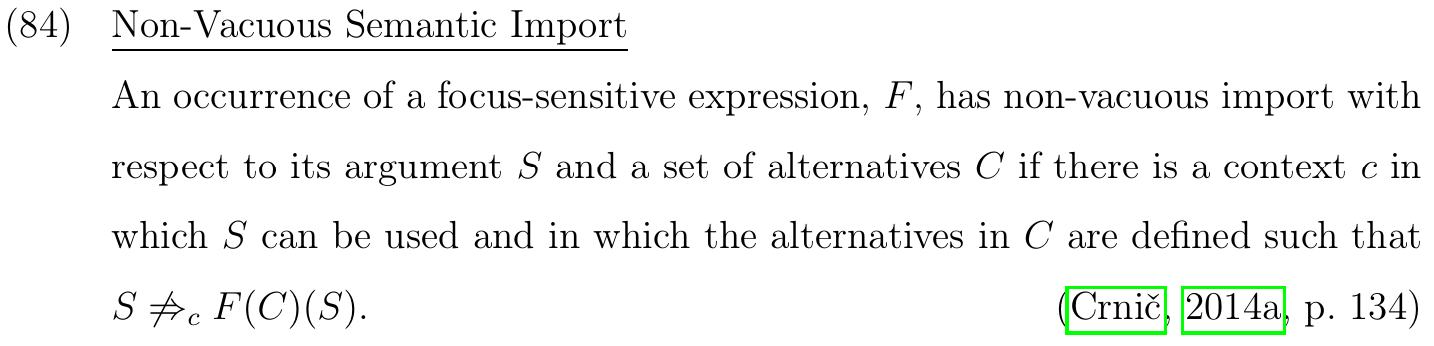
\includegraphics[width=0.8\textwidth]{graphics/crnic-semanticimport.png}
\end{figure}\vfill
\end{frame}

\begin{frame}[t]
    \subsectionpage\vskip 9pt\vfill
\begin{figure}
    \centering
    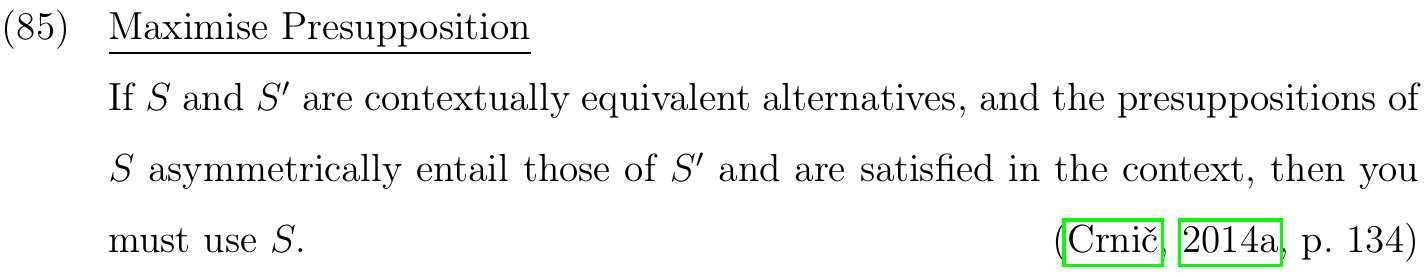
\includegraphics[width=0.8\textwidth]{graphics/crnic-maximisepresupposition.png}
\end{figure}\vfill
\end{frame}

\subsection{NPI Questions}
\begin{frame}[t]
    \subsectionpage\vskip 9pt\vfill
\begin{figure}
    \centering
    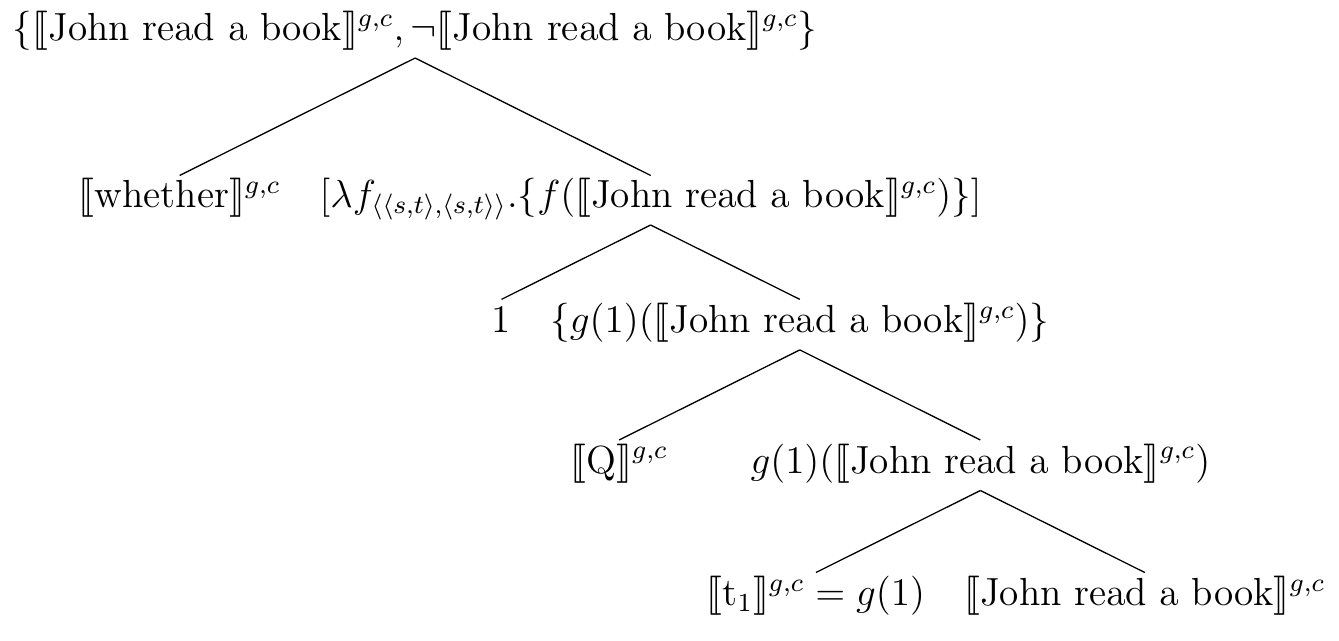
\includegraphics[height=8cm]{graphics/questions-guerzoni2003.png}
    \caption{Answers to Question Approach Tree}
\end{figure}\vfill
\end{frame}

\begin{frame}[t]
    \subsectionpage\vskip 9pt\vfill
\begin{figure}
    \centering
    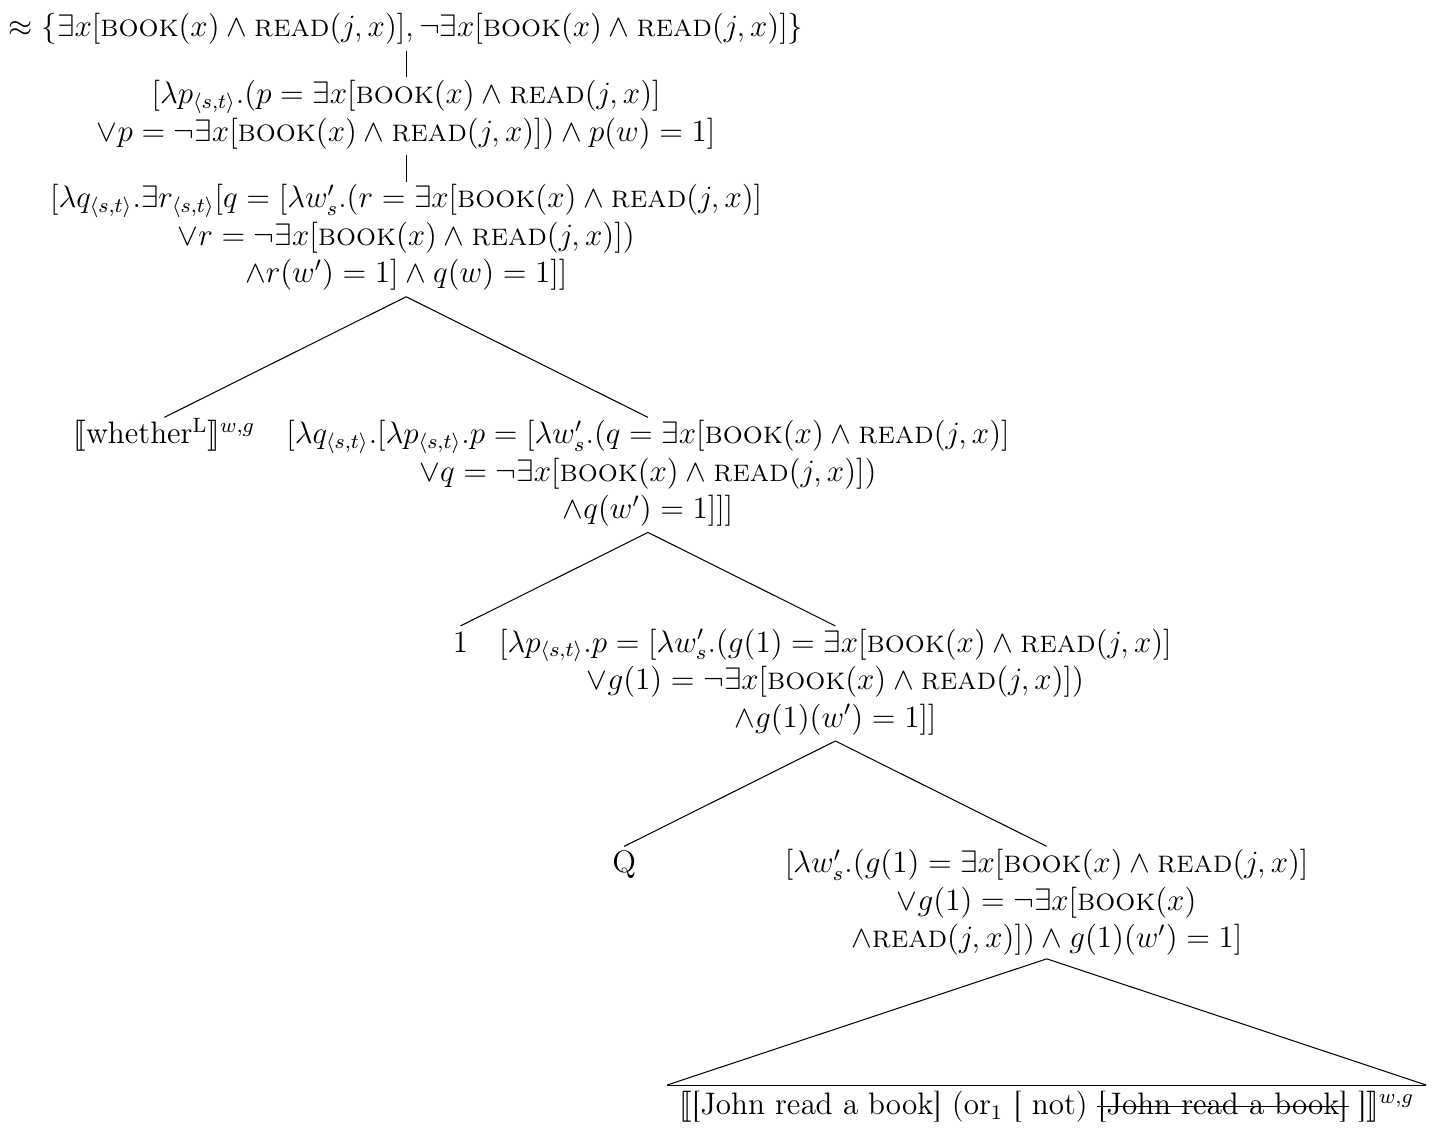
\includegraphics[height=8cm]{graphics/questions-guerzonisharvit2014.png}
    \caption{Environments in Questions Approach}
\end{figure}\vfill
\end{frame}